\documentclass[border=10pt]{standalone}

\usepackage{tikz}
\usepackage{tikzsymbols}
\usetikzlibrary{calc,patterns,shapes.geometric}

\def\centerarc[#1](#2)(#3:#4:#5){\draw[#1] ($(#2)+({#5*cos(#3)},{#5*sin(#3)})$) arc (#3:#4:#5);}

\begin{document}
	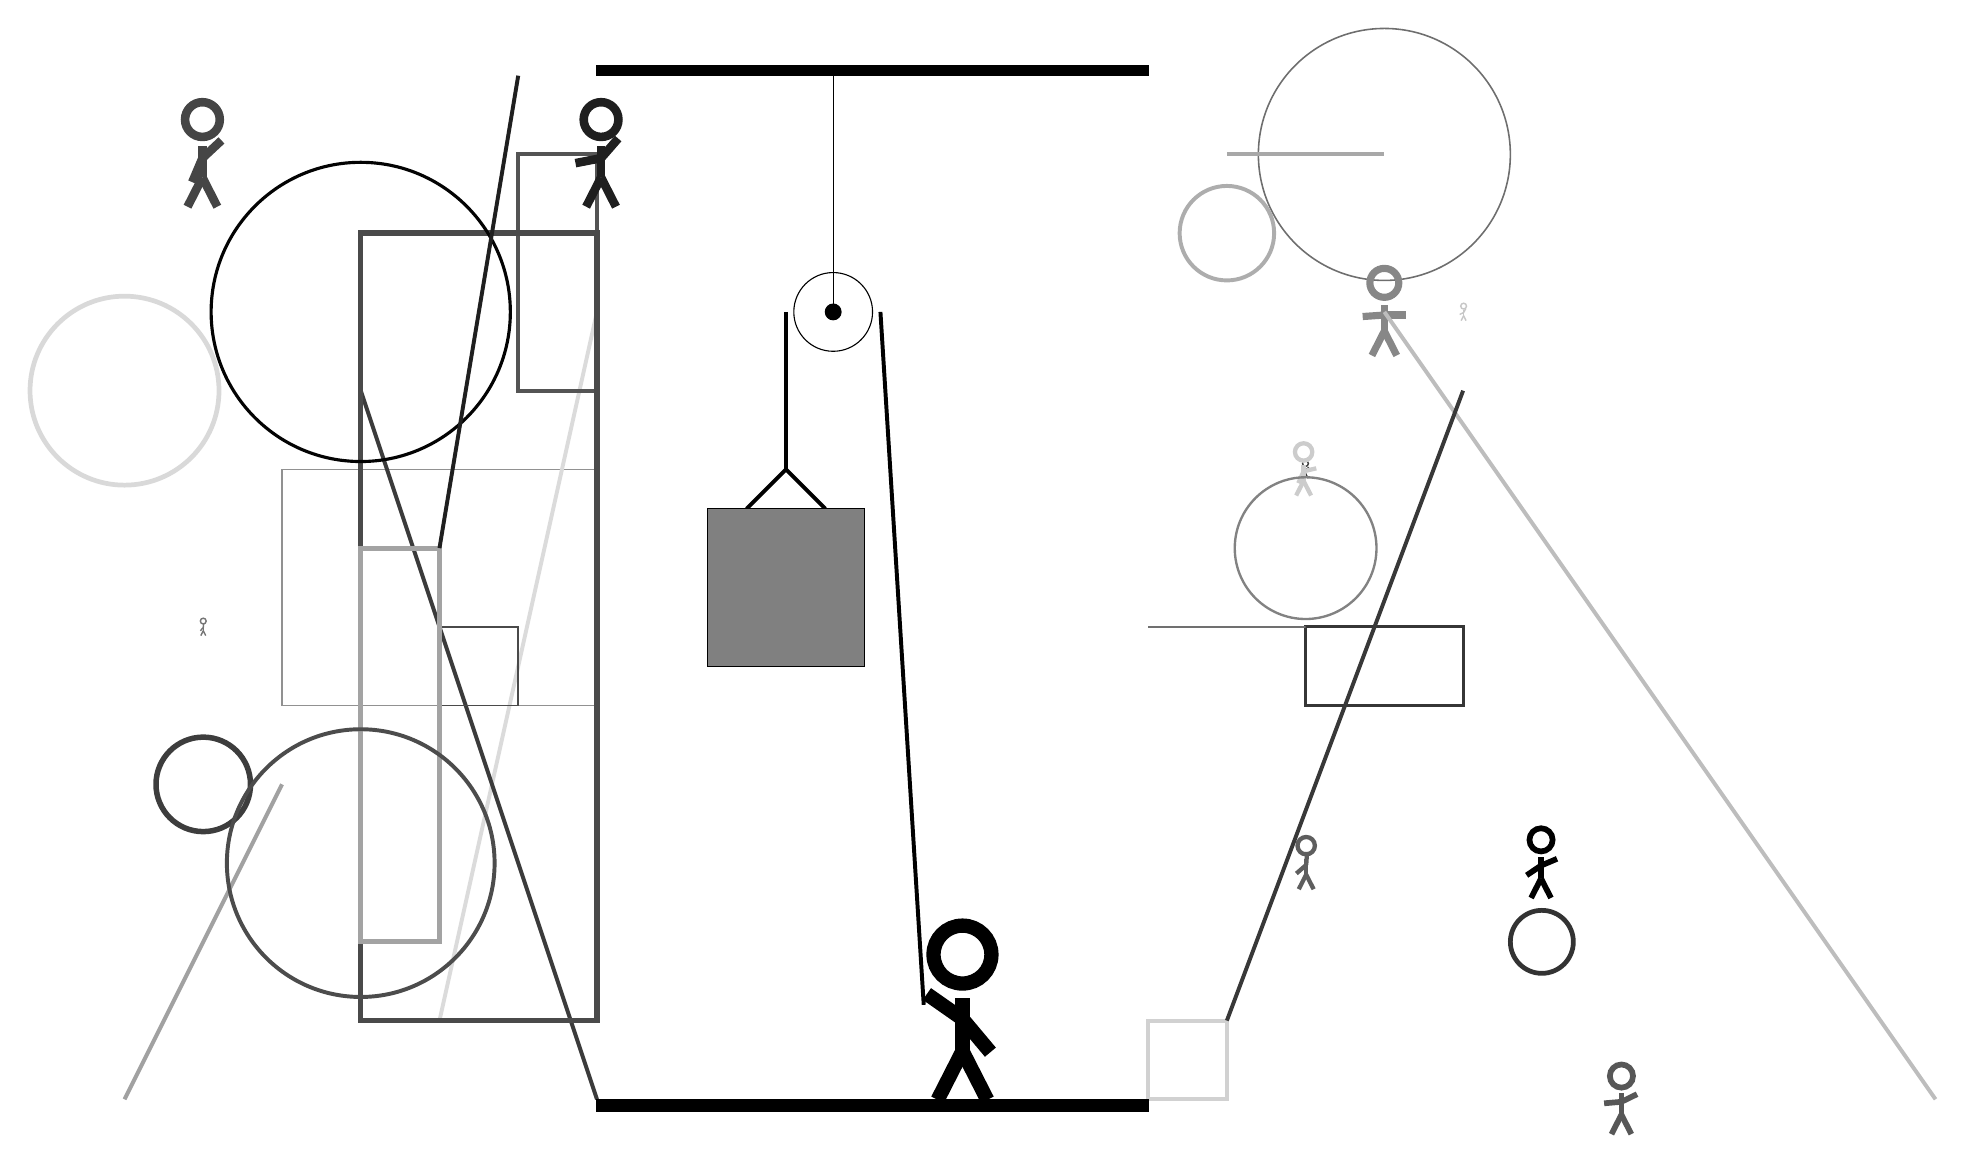
\begin{tikzpicture}
		%%%%% START %%%%%
		
		\draw[fill=black] (-2, 10) rectangle (5, 10.125);
		
		\draw (1, 7) circle (0.5);
		\draw[fill=black] (1, 7) circle (0.1);
		\draw (1, 10) -- (1, 7);
		
		\draw[line width=0.5mm] (-0.1, 4.5) -- (0.4, 5.0) -- (0.9, 4.5);
		\draw[fill=black!50] (-0.6, 4.5) rectangle (1.4, 2.5);
		
		\draw [line width=0.5mm, color=black!51](8, 8) circle (0.0);
		
		\draw [line width=0.2mm, color=black!57](8, 9) circle (1.6);
		\node[line width=0.3mm, color=black!54] at (-7, 3) {\Strichmaxerl[1][49][84]};
		\draw[line width=0.5mm, color=black!37](-6, 1) -- (-8, -3);
		\draw[line width=0.2mm, color=black!43] (-2, 2) rectangle (-6, 5);
		\draw[line width=0.5mm, color=black!33](-5, 1) -- (-5, 8);
		
		\draw[line width=0.5mm, color=black!14](-4, -2) -- (-2, 7);
		\draw[line width=0.5mm, color=black!67] (-2, 6) rectangle (-3, 9);
		\draw [line width=0.5mm, color=black!32](6, 8) circle (0.6);
		\node[line width=0.6mm, color=black!63] at (7, 0) {\Strichmaxerl[3][41][86]};
		\draw[line width=0.5mm, color=black!34](6, 9) -- (8, 9);
		
		\node[line width=0.2mm, color=black!66] at (11, -3) {\Strichmaxerl[4][5][26]};
		\draw[line width=0.5mm, color=black!77](-5, 6) -- (-2, -3);
		
		\node[line width=0.7mm, color=black!76] at (7, 5) {\Strichmaxerl[1][45][39]};
		\node[line width=0.2mm, color=black!100] at (10, 0) {\Strichmaxerl[4][34][23]};
		\node[line width=0.2mm, color=black!20] at (7, 5) {\Strichmaxerl[3][66][13]};
		
		\node[line width=0.4mm, color=black!73] at (-7, 9) {\Strichmaxerl[6][67][43]};
		\draw [line width=0.6mm, color=black!80](10, -1) circle (0.4);
		\draw [line width=0.3mm, color=black!49](7, 4) circle (0.9);
		\draw[line width=0.2mm, color=black!71] (-4, 3) rectangle (-3, 2);
		\node[line width=0.6mm, color=black!47] at (8, 7) {\Strichmaxerl[5][4][0]};
		
		\draw[line width=0.7mm, color=black!71] (-2, -2) rectangle (-5, 8);
		
		\draw[line width=0.6mm, color=black!36] (-4, -1) rectangle (-5, 4);
		\draw [line width=0.6mm, color=black!15](-8, 6) circle (1.2);
		\draw[line width=0.5mm, color=black!18] (5, -3) rectangle (6, -2);
		\node[line width=0.2mm, color=black!22] at (9, 7) {\Strichmaxerl[1][26][61]};
		\draw [line width=0.7mm, color=black!76](-7, 1) circle (0.6);
		\draw [line width=0.4mm, color=black!99](-5, 7) circle (1.9);
		\draw [line width=0.5mm, color=black!70](-5, 0) circle (1.7);
		
		\draw[line width=0.5mm, color=black!26](8, 7) -- (15, -3);
		\draw[line width=0.4mm, color=black!79] (7, 3) rectangle (9, 2);
		
		\node[line width=0.6mm, color=black!88] at (-2, 9) {\Strichmaxerl[6][11][49]};
		\draw[line width=0.2mm, color=black!56] (5, 3) rectangle (7, 3);
		
		\draw[line width=0.5mm, color=black!78](6, -2) -- (9, 6);
		\draw[line width=0.5mm, color=black!88](-3, 10) -- (-4, 4);
		
		\draw[line width=0.5mm] (0.4, 7) -- (0.4, 5.0);
		\centerarc[line width=0.5mm](1, 7)(0:180:0.6);
		\draw[line width=0.5mm](1.6, 7) -- (2.15, -1.8);
		
		\node at (2.6, -1.9) {\Strichmaxerl[10][-35][-50]};
		
		\draw[fill=black] (-2, -3) rectangle (5, -3.15);
		
		%%%%% END %%%%%
	\end{tikzpicture}
\end{document}